

\chapter{Overview dell'architettura e delle componenti utilizzate \workinprogress}

\label{ch:overview}

\section{Obbiettivo da ottenere \workinprogress}
\label{sec:overview-goal}

In una collaborazione tra il Dipartimento di Ingegneria dell'Informazione e l'azienda \textbf{Esse-ti S.R.L.} ci è stato esposto un progetto che consiste nel:


\begin{itemize}[nosep, itemsep=0.2em]
	\item Fornire a dei clienti un router 4G, su cui possono essere connessi vari dispositivi, ad es. di tipo domotico;
	\item Rendere questi dispositivi accessibili ai clienti attraverso internet;
\end{itemize}

\begin{figure}[H]
	\centering
	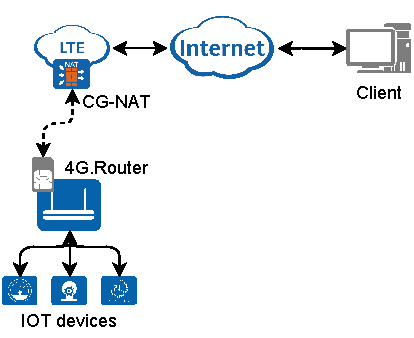
\includegraphics[width=0.5\linewidth]{immagini/diag-goal}
	\caption{Schema concettuale dell'obbiettivo da raggiungere.}
	\label{fig:schema_concettuale}
\end{figure}

E' pratica comune degli operatori mobili di implemtare nella loro rete un CG-NAT (sezione~\ref{subsubsec:cg-nat}) per gestire il traffico degli utenti, ciò significa che la comunicazione da internet verso il \textit{router} non è possibile in generale. Un modo per risolvere questo problema potrebbe essere di richiede al cliente di avere a disposizione un IP pubblico, ciò però non è sempre possibile e sarebbe molto scomodo per il cliente. 

Quindi per una soluzione più generale a questa topologia si deve necessariamente introdurre una terza macchina provvista di IP pubblico e che funga da ponte tra il \textit{4G.Router} e il cliente.


\begin{figure}[H]
	\centering
	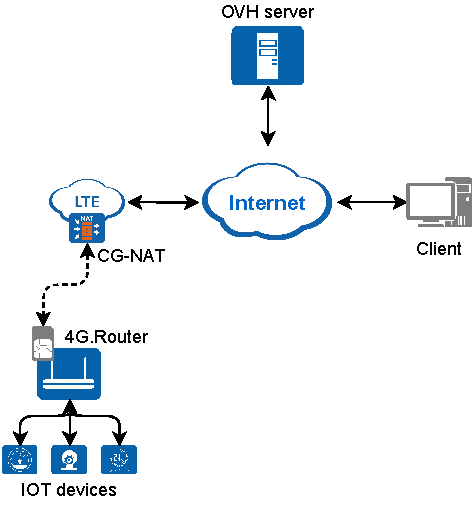
\includegraphics[width=0.5\linewidth]{immagini/diag-real}
	\caption{Schema concettuale dell'architettura che si dovrà implementare.}
	\label{fig:schem_architettura_reale}
\end{figure}

In questo modo si può usare il \textit{Server OVH} per configurare una \textit{Virtual Private Network} (VPN), a cui saranno connessi sia il \textit{4G.Router} che il cliente. Ciò consente la creazione di una topologia virtuale in cui tutti i dispositivi connessi alla VPN sono nella stessa rete locale, quindi possono comunicare tra loro.

Inoltre in questo modo viene minimizzata la configurazione da effettuare sulle macchine dei clienti, sarà infatti sufficiente avere un client OpenVPN.

La configurazione virtuale vista dal 4G.Router e dai clienti sarà quindi:

\begin{figure}[H]
	\centering
	\includegraphics[width=0.5\linewidth]{immagini/diag-virtual}
	\caption{Topologia virtuale vista dal cliente.}
	\label{fig:schema_architettura_virtuale}
\end{figure}

\newpage
\section{Specifiche dei componenti}

\subsubsection{VPS OVHCloud}
\label{subsec:vps-ovhcloud}

\todo[leva abbastanza]
La VPS ha il solo vincolo di dover avere un'IP pubblico e una connessione a internet abbastanza veloce. Dovrà infatti sopportare un traffico simmetrico in upload/download.

Per la realizzazione della topologia è stata selezionata una macchina VPS del provider \textit{OVHCloud}, con le seguenti caratteristiche:


\begin{itemize}[nosep]
	\item 2 core virtuali;
	\item 4Gb di memoria ram;
	\item 80Gb di storage NVMe;
	\item 500Mbps simmetrici di banda;
	\item ipv4 pubblico;
	\item Ubuntu 16.04;
\end{itemize}

Per semplicità si farà riferimento alla \textit{VPS OVHCloud} come \textit{Server}.

\subsubsection{Esse-ti 4G.Router}

Ci è stato fornito dall'azienda Esse-ti, consiste in un gateway 4G con funzionalità di router. Le specifiche complete possono essere trovate sul sito del produttore (\href{https://www.esse-ti.it/4g-router}{link}).


\begin{figure}[ht]
	\centering
	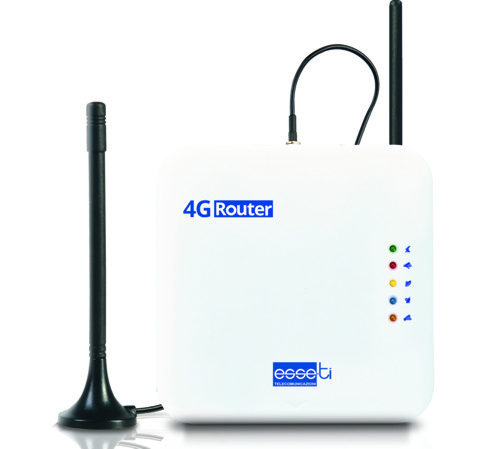
\includegraphics[width=240px]{immagini/4grouter.jpg}
	\caption{Esse-ti 4G.Router}
	\label{fig:esse-ti-router-4g}
\end{figure}

Per l'implementazione di questa architettura sono necessarie solo un sub-set delle specifiche:

\begin{itemize}[nosep]
	\item Modulo LTE per consentire l'accesso a internet;
	\item Porta LAN e Access Point Wi-Fi;
\end{itemize}

\newpage
Il sistema operativo del router è una versione personalizzata di OpenWRT, le funzionalità sono le stesse della versione OpenSource ma la grafica è leggermente differente ed è preconfigurato con le impostazioni per la gestione del 4G.

% ok
La configurazione del dispositivo può essere fatta sia da terminale, entrando in ssh, sia da interfaccia web:

\begin{figure}[H]

	\newlength{\tempheight}
	\setlength{\tempheight}{23ex}

	\centering%
	\begin{subfigure}[t]{0.5\textwidth}
		\centering%
		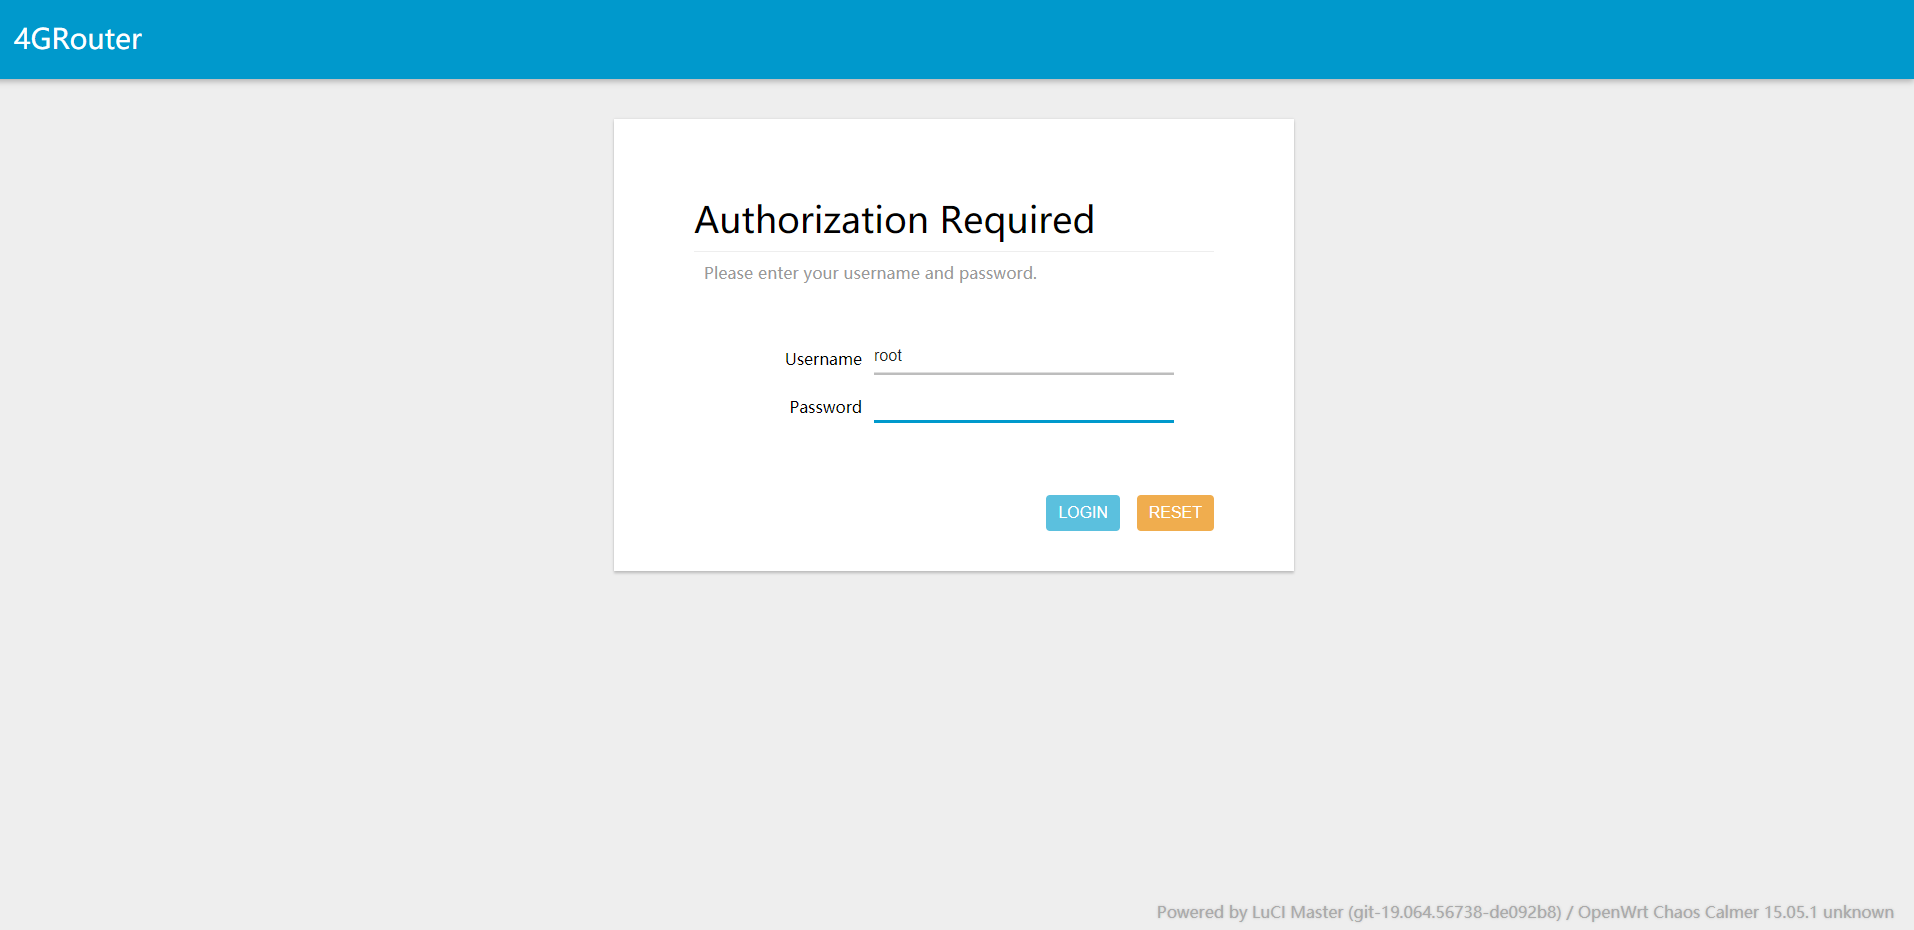
\includegraphics[totalheight=\tempheight]{immagini/interfacciar4g_init}
		\caption{Schermata di autenticazione}
	\end{subfigure}%
	\hfill
	\begin{subfigure}[t]{0.5\textwidth}
		\centering%
		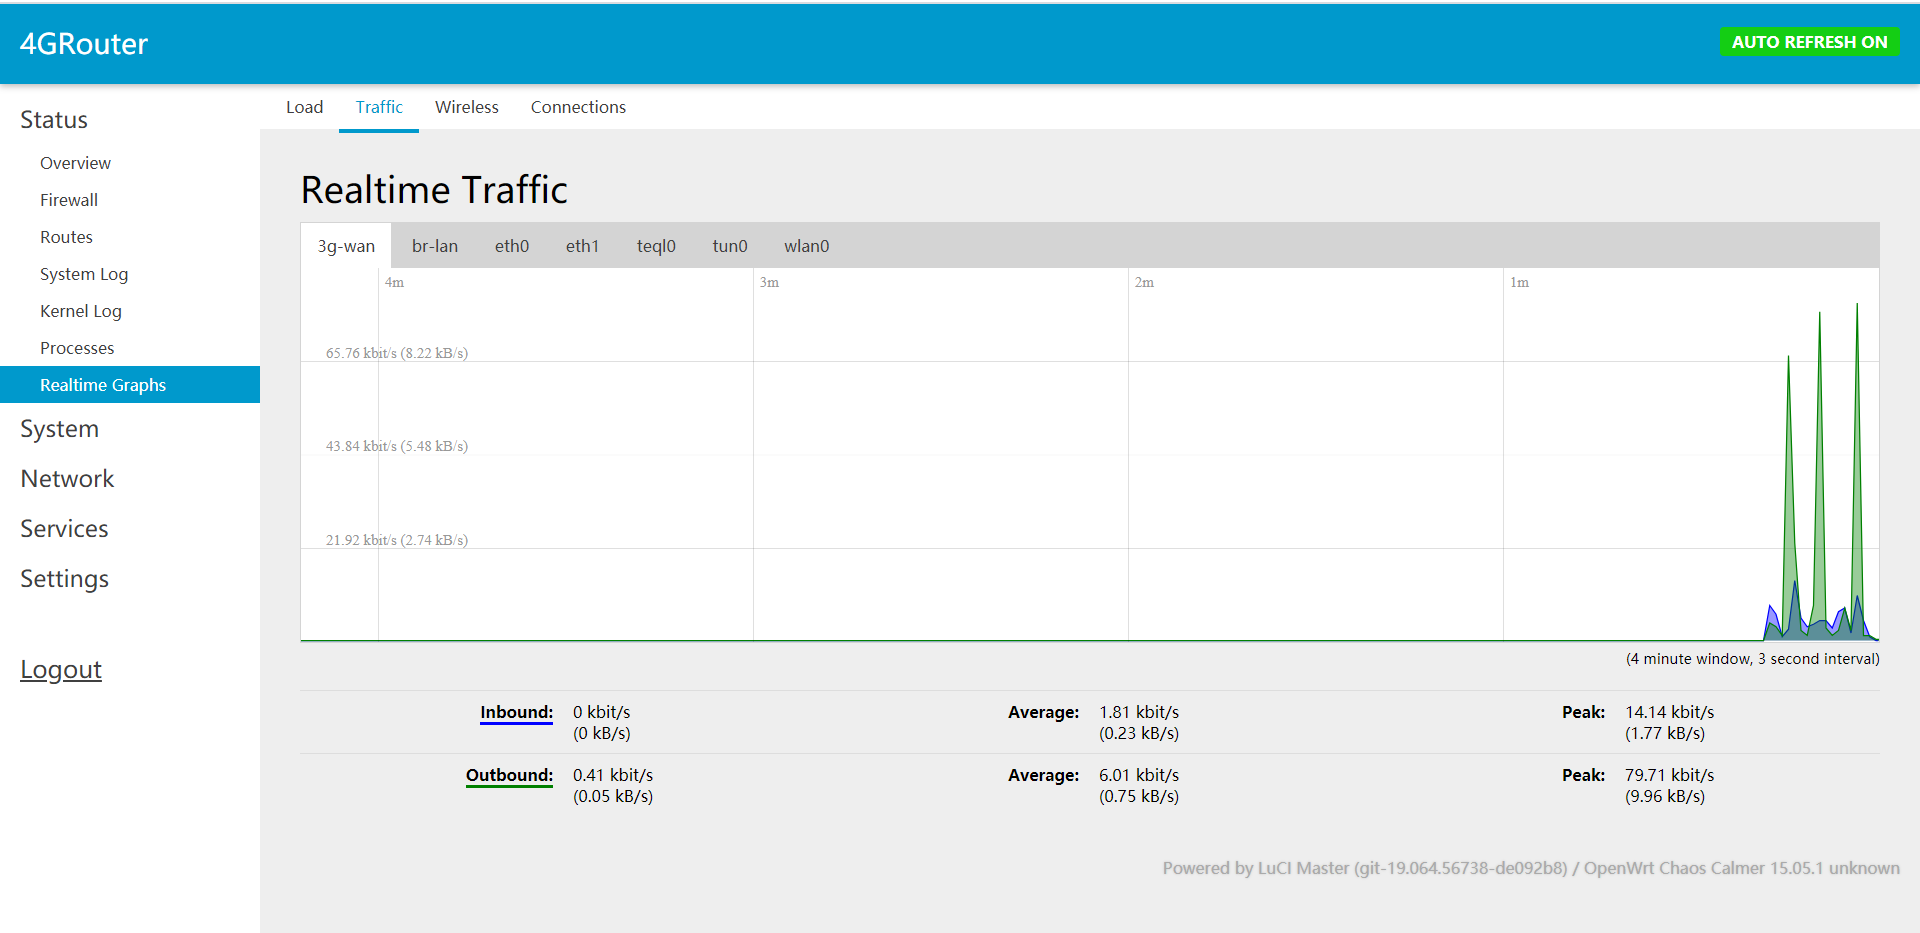
\includegraphics[totalheight=\tempheight]{immagini/interfacciar4g_traffic}
		\caption{Grafico del traffico}
	\end{subfigure}

	\medskip

	\begin{subfigure}[b]{\textwidth}
		\centering%
		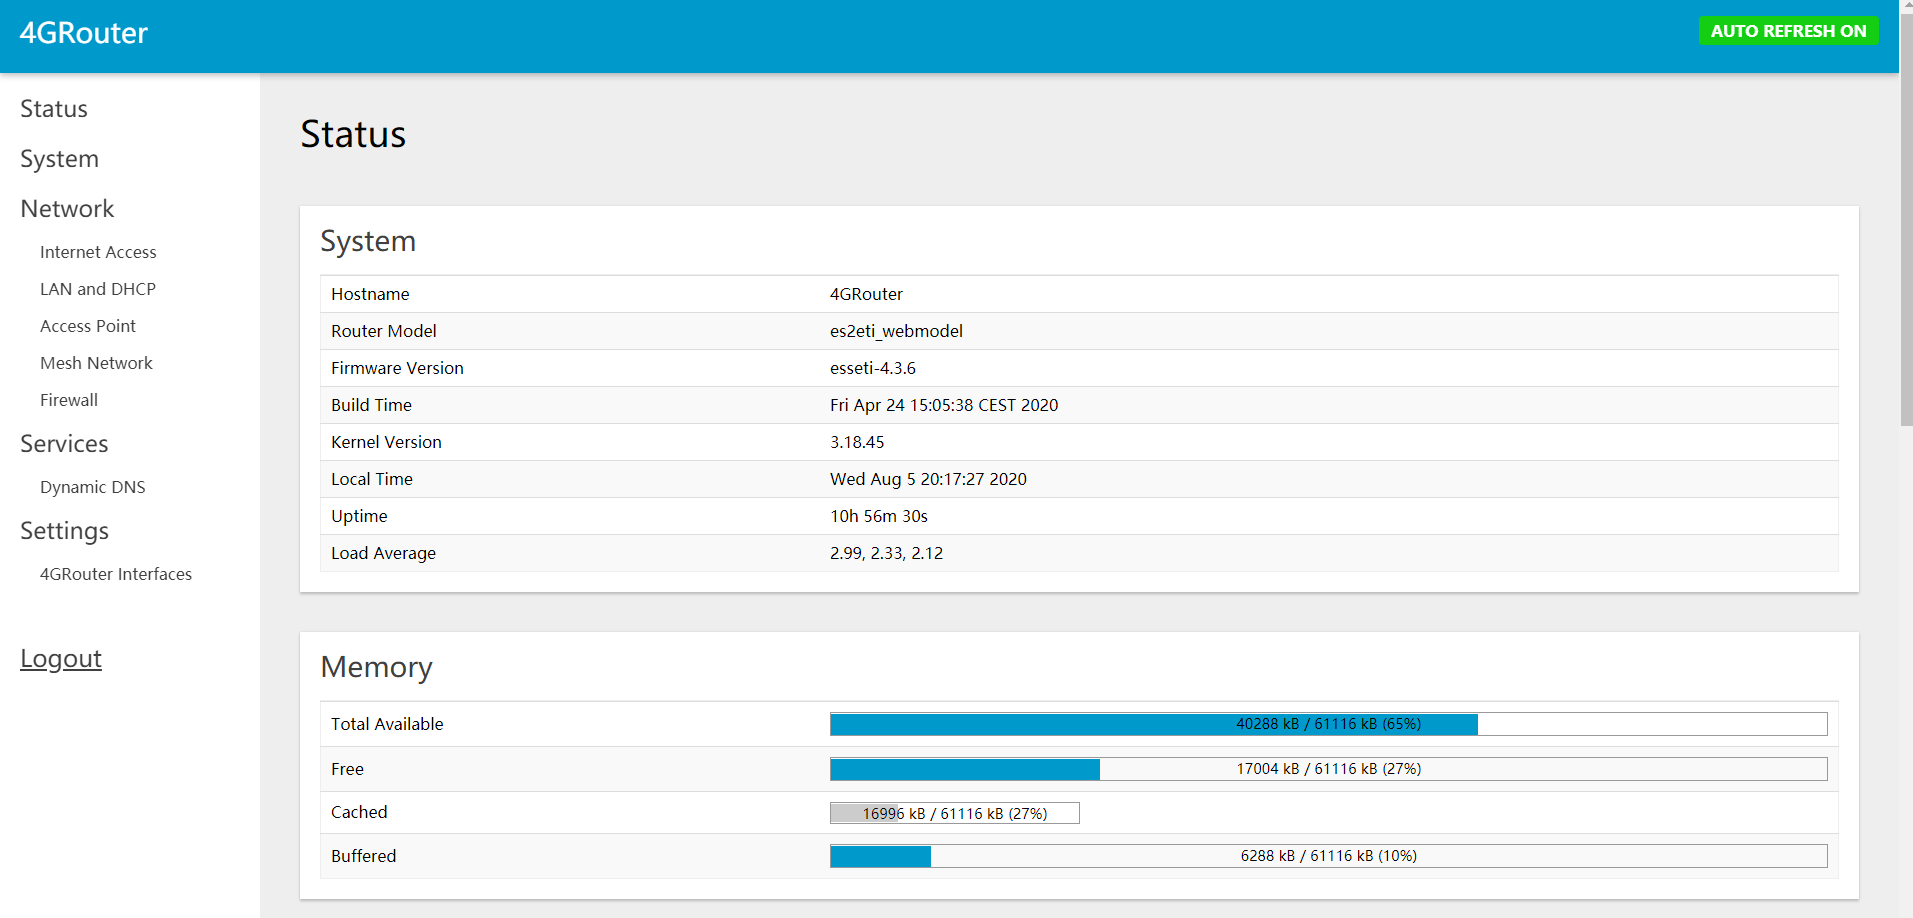
\includegraphics[totalheight=2\tempheight]{immagini/interfacciar4g_status}
		\caption{Schermata con stato riassuntivo}
	\end{subfigure}
	\caption{Interfaccia web Esse-ti 4G.Router}

\end{figure}

Per semplicità si farà riferimento all'\textit{Esse-ti 4G.Router} chiamandolo semplicemente \textit{Router}.

\subsubsection{Macchina del cliente}
\label{subsec:macchina-cliente}

Per avere la massima flessibilità la macchina del cliente deve essere generica e non deve necessitare di nessuna configurazione specifica, essendo OpnenVPN un applicativo cross-platform ci consente si non avere vincoli di sistema operativo.

Si farà riferimento a una generica macchina di un cliente come \textit{Client}.

\newpage
\subsubsection{Host domotico}

L'obbiettivo dell'azienda \textit{Esse-ti} è quello di fornire ai clienti una connessione diretta verso dispositivi domotici posti in una locazione remota. In questa topologia un'\textit{host-domotico} potrebbe essere un qualunque dispositivo di rete, ad es: una telecamera di videosorveglianza, un termostato digitale o un dispositivo più complesso come una \href{https://en.wikipedia.org/wiki/Raspberry_Pi}{Raspberry Pi}.

Per simulare un'\textit{host-domotico} ed effettuare le varie operazioni di testing è stata usata una \textit{Raspberry Pi}.


